
\section{Manual de despliegue e instalación} 

Para utilizar la aplicación se puede acceder al enlace de la aplicación Web que se encuentra en el Apéndice \ref{anexoenlaces}.

\subsection{Requisitos para la instalación}
En caso de que se quiera desplegar la aplicación en local, se debe tener instalado el siguiente \textit{software}:
\begin{itemize}
    \item Angular: versión 15.1.4 o superior.
    \item NodeJS: versión 18.14.0 o superior.
    \item Git: versión 2.35.1 o superior en caso de que se quiera clonar el repositorio.
    \item MySQL Workbench: versión 8.0.32 o superior.
\end{itemize} 


\subsection{Instalación}
Los pasos a seguir para desplegar el proyecto son los siguientes:
\begin{itemize}
    \item Descargar el código del proyecto del repositorio de Gitlab que se encuentra en el Apendice \ref{anexoenlaces}. Para ello se puede descargar el .zip con el código del proyecto o clonar el repositorio mediante el comando:
    
         \textbf{\texttt{\$  git clone https://gitlab.inf.uva.es/josloza/tfg-josloza}   }                   
      
       
   
    \item En la carpeta \texttt{frontend} que contiene el código de la parte de Angular, se debe ejecutar en un terminal el siguiente comando para instalar las dependencias necesarias para que la parte de Angular funcione:
    
      \textbf{\texttt{\$  npm install}   } 
      
        
    
    \item A continuación en la misma carpeta se debe ejecutar el siguiente comando para desplegar la parte de Angular:
   
       \textbf{\texttt{\$  ng serve}   }  
      
        

        \item En la carpeta \texttt{backend} se debe ejecutar en un terminal el siguiente comando para instalar las dependencias necesarias para que la parte de NodeJS funcione:
      
          \textbf{\texttt{\$  npm install}   }  

        \item A continuación, en la misma carpeta se debe ejecutar el siguiente comando para desplegar la parte de NodeJS:
        
            \textbf{\texttt{\$  node index.js}   }  

        \item Una vez hecho esto, se puede acceder desde un navegador a la url \url{http://localhost:4200/} que mostrará la aplicación Web en funcionamiento.
        
\end{itemize}




    




    



\section{Manual de Usuario}

Se han tratado de realizar interfaces intuitivas y fáciles de utilizar para que el Usuario aprenda rápidamente su manejo. Sin embargo, a continuación se explican los pasos que puede realizar un Usuario al utilizar la aplicación y cómo puede interactuar con las pantallas.

\subsection{Registro e inicio de sesión}

Al entrar al enlace de la aplicación definido en Apéndice \ref{anexoenlaces}, se muestra la \textbf{pantalla descripcion-aplicacion} (Figura \ref{fig:ma-descripcion-aplicacion}) donde se describe la funcionalidad de la aplicación. En esta pantalla si se pulsa sobre el botón \textit{registro}, se dirigirá al Usuario a la \textbf{pantalla registro-usuario} (Figura \ref{fig:ma-registro}) para registrarse en la aplicación. Una vez registrado, desde la pantalla descripcion-aplicacion si se pulsa el botón \textit{identificarse} se le dirigirá a la \textbf{pantalla identificacion-usuario} (Figura \ref{fig:ma-identificacion}) para identificarse donde se puede identificar en la aplicación con el \textit{username} y contraseña que se ha introducido en el registro.

\subsection{Muro publicaciones, datos del Usuario y su edición}

Una vez identificado, se mostrará la \textbf{pantalla muro-publicaciones} (Figura \ref{fig:ma-muro-publicaciones}) que no mostrará ninguna publicación ya que todavía no se sigue a ningún usuario. En la barra de navegación de la parte superior de esta pantalla si se pulsa sobre \textit{mi perfil} se le llevará a la \textbf{pantalla perfil-usuario} (Figura \ref{fig:ma-perfil-usuario}) donde se muestran los datos de su perfil. Una vez ahí, si se pulsa sobre el botón \textit{editar perfil} se accederá a la \textbf{pantalla editar-usuario} (Figura \ref{fig:ma-editar-usuario}) para editar los datos del perfil donde se puede cambiar la foto de perfil o contraseña entre otros datos. Una vez hechos los cambios si se pulsa el botón \textit{guardar} se le dirigirá de vuelta a la pantalla perfil-usuario donde se muestran los datos de su perfil actualizados.

\subsection{Buscador de usuarios, detalles del Usuario y seguidos}

En la barra de navegación superior, si se pulsa sobre \textit{buscar} aparecerá un menú despegable. Si se pulsa sobre \textit{buscar usuario} se abrirá la \textbf{pantalla buscar-usuario} (Figura \ref{fig:ma-buscar-usuario}) para buscar usuarios donde se podrá introducir un \textit{username} para buscar. Si se clica sobre la carta de un Usuario se mostrarán los detalles del Usuario en la \textbf{pantalla detalles-usuario} (Figura \ref{fig:ma-detalles-usuario}). Si se pulsa el botón \textit{seguir usuario} se comenzará a seguir al Usuario y en la pantalla perfil-usuario pulsando sobre el número de usuarios seguidos se le dirigirá a la \textbf{pantalla seguidos-usuario} (Figura \ref{fig:ma-seguidos-usuario}) que muestra los usuarios a los que sigue. Si en cambio en la pantalla perfil-usuario se pulsa sobre el número de seguidores, se le dirigirá a la \textbf{pantalla seguidores-usuario} (Figura \ref{fig:ma-seguidores-usuario}) donde se mostrarán los usuarios que le siguen.

\subsection{Buscador de recetas, detalles de la receta y favoritas}

En el menú despegable al pulsar \textit{buscar} si se pulsa sobre \textit{buscar receta} se le abrirá la \textbf{pantalla buscar-receta} (Figura \ref{fig:ma-buscar-receta}). En ella se puede introducir el título de la receta a buscar y al clicar sobre una carta de una receta se mostrará la \textbf{pantalla detalles-receta} (Figura \ref{fig:ma-detalles-receta}) con los detalles de la receta. En esta pantalla se puede pulsar el botón \textit{añadir receta a favoritas} para añadir la receta a favoritas y en la pantalla perfil-usuario pulsando sobre el botón \textit{mis recetas favoritas}, se le dirigirá a la \textbf{pantalla favoritas-recetas} (Figura \ref{fig:ma-favoritas-recetas}) que muestra las recetas favoritas del Usuario donde se incluirá esta receta. 

\subsection{Buscador de alimentos y detalles del alimento}

En el menú despegable al pulsar \textit{buscar} si se pulsa sobre \textit{buscar alimento}, se abrirá la \textbf{pantalla buscar-alimento} (Figura \ref{fig:ma-buscar-alimento}). Aquí se podrá introducir el nombre del alimento que desea buscar y clicando sobre una carta de un alimento, se mostrará la \textbf{pantalla detalles-alimento} (Figura \ref{fig:ma-detalles-alimento}) con los detalles del alimento.

\subsection{Crear receta y crear publicación}

En la barra de navegación superior, si se pulsa sobre \textit{crear} aparecerá un menú despegable. Si se pulsa sobre \textit{crear receta} se dirigirá al Usuario a la \textbf{pantalla crear-receta} (Figura \ref{fig:ma-crear-receta}). En esta pantalla, si se rellenan todos los campos se podrá crear una receta. En cambio si en el menú despegable al pulsar \textit{crear} se pulsa en \textit{crear publicación} se le dirigirá a la \textbf{pantalla crear-publicacion} (Figura \ref{fig:ma-crear-publicacion}). De la misma forma, introduciendo los valores requeridos, se podrá crear una publicación. 


\subsection{Administrador}

Si el Usuario al identificarse tiene el rol de Administrador, se le dirigirá a la \textbf{pantalla vista-admin} (Figura \ref{fig:ma-usuarios-admin}). En ella, aparecen por defecto todos los usuarios registrados en la aplicación. Si se clica en la pestaña \textit{alimentos}, se mostrarán todos los alimentos almacenados en la aplicación (Figura \ref{fig:ma-alimentos-admin}). Si se clica en la pestaña \textit{recetas}, se mostrarán todas las recetas creadas en la aplicación (Figura \ref{fig:ma-recetas-admin}). Si se clica en la pestaña \textit{publicaciones}, se mostrarán todas las publicaciones hechas en la aplicación (Figura \ref{fig:ma-publicaciones-admin}). Estas pantallas se muestran como una tabla donde las filas son los elementos de cada tipo. Se puede eliminar cualquiera de estos elementos, pulsando sobre el botón \textit{eliminar} en la fila que corresponda al elemento. 

\subsection{Crear alimento y editar}

Por otro lado, desde la pantalla vista-admin, si se pulsa el botón \textit{crear alimento}, se mostrará la \textbf{pantalla crear-alimento} (Figura \ref{fig:ma-crear-alimento}). En ella, rellenado los campos se podrá crear un alimento. Sin embargo, si quiere editar un alimento, clicando sobre la pestaña de alimentos en la pantalla vista-admin, se puede pulsar el botón \textit{editar} sobre el alimento que desee. A continuación, se abrirá la pantalla crear-alimento pero cargando los datos del alimento a editar (Figura \ref{fig:ma-editar-alimento}).


\begin{figure}[H]
  \centering
  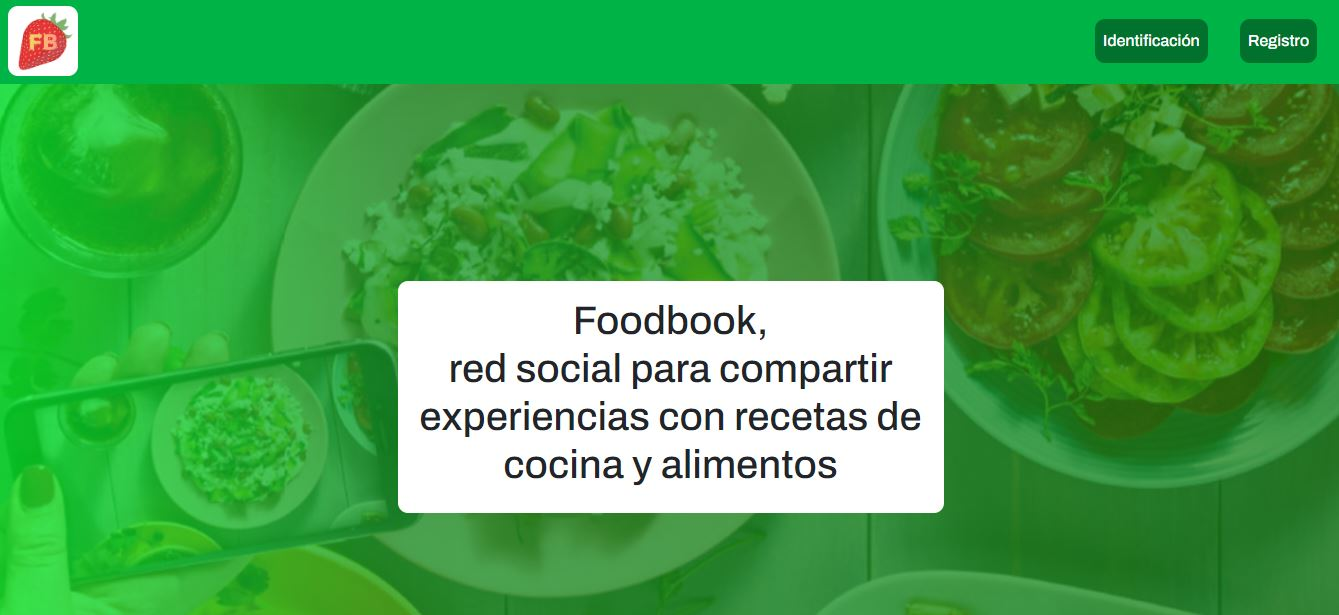
\includegraphics[scale=0.30]{img/ma-descripcion-aplicacion.JPG}
  \caption{Pantalla descripcion-aplicacion.}
  \label{fig:ma-descripcion-aplicacion}
\end{figure}

\begin{figure}
  \centering
  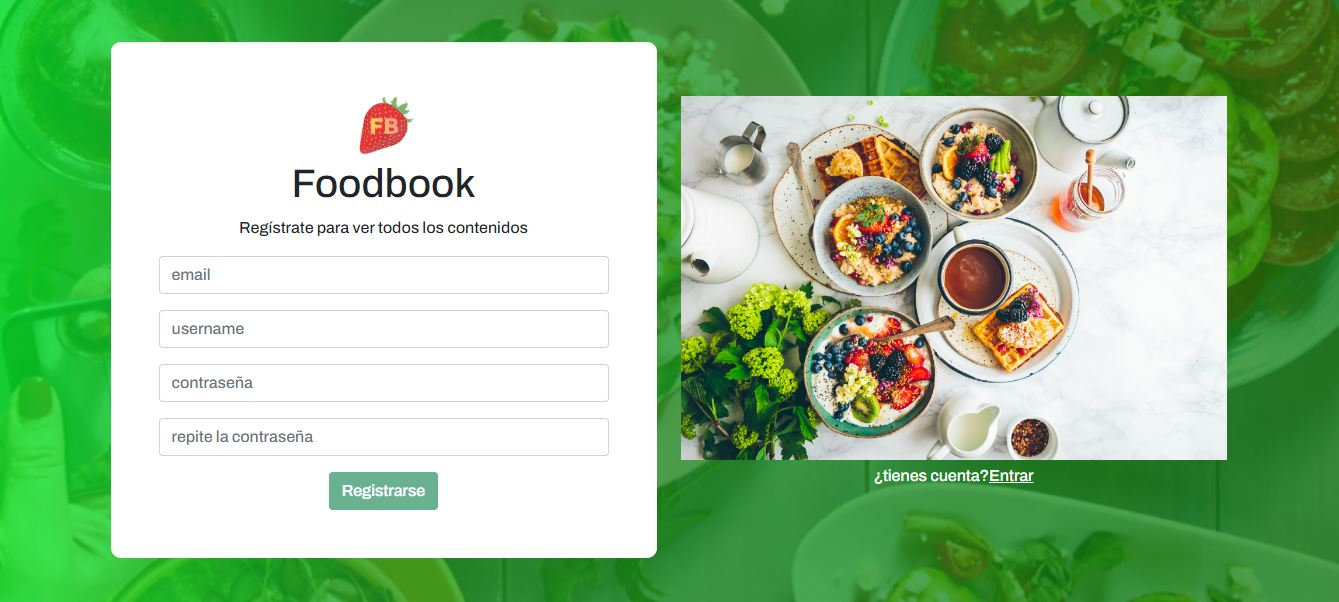
\includegraphics[scale=0.30]{img/ma-registro.JPG}
  \caption{Pantalla registro-usuario.}
  \label{fig:ma-registro}
\end{figure}

\begin{figure}
  \centering
  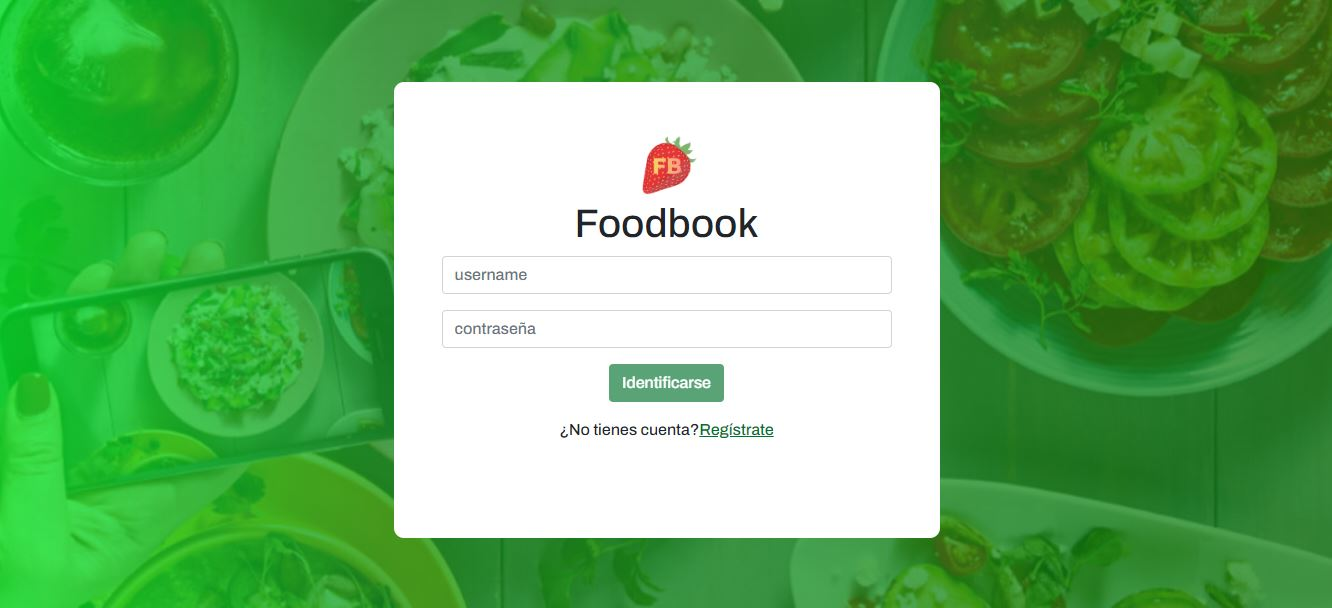
\includegraphics[scale=0.30]{img/ma-identificacion.JPG}
  \caption{Pantalla identificacion-usuario.}
  \label{fig:ma-identificacion}
\end{figure}





\begin{figure}
  \centering
  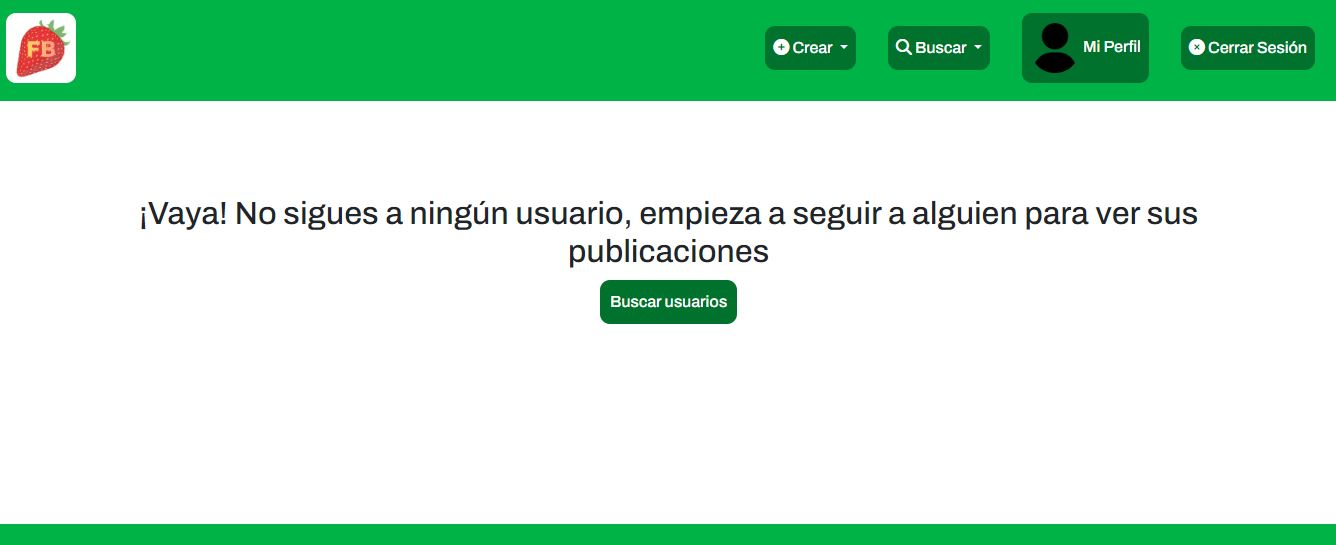
\includegraphics[scale=0.30]{img/ma-muro-publicaciones.JPG}
  \caption{Pantalla muro-publicaciones.}
  \label{fig:ma-muro-publicaciones}
\end{figure}

\begin{figure}
  \centering
  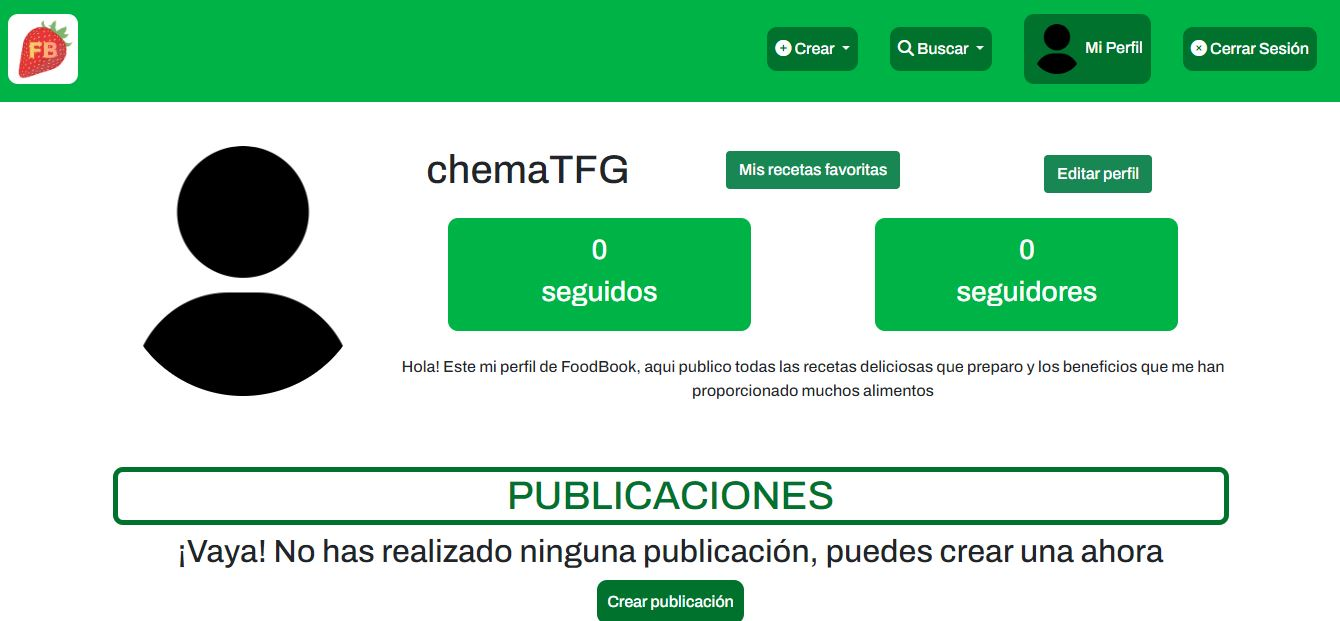
\includegraphics[scale=0.30]{img/ma-perfil-usuario.JPG}
  \caption{Pantalla perfil-usuario.}
  \label{fig:ma-perfil-usuario}
\end{figure}

\begin{figure}
  \centering
  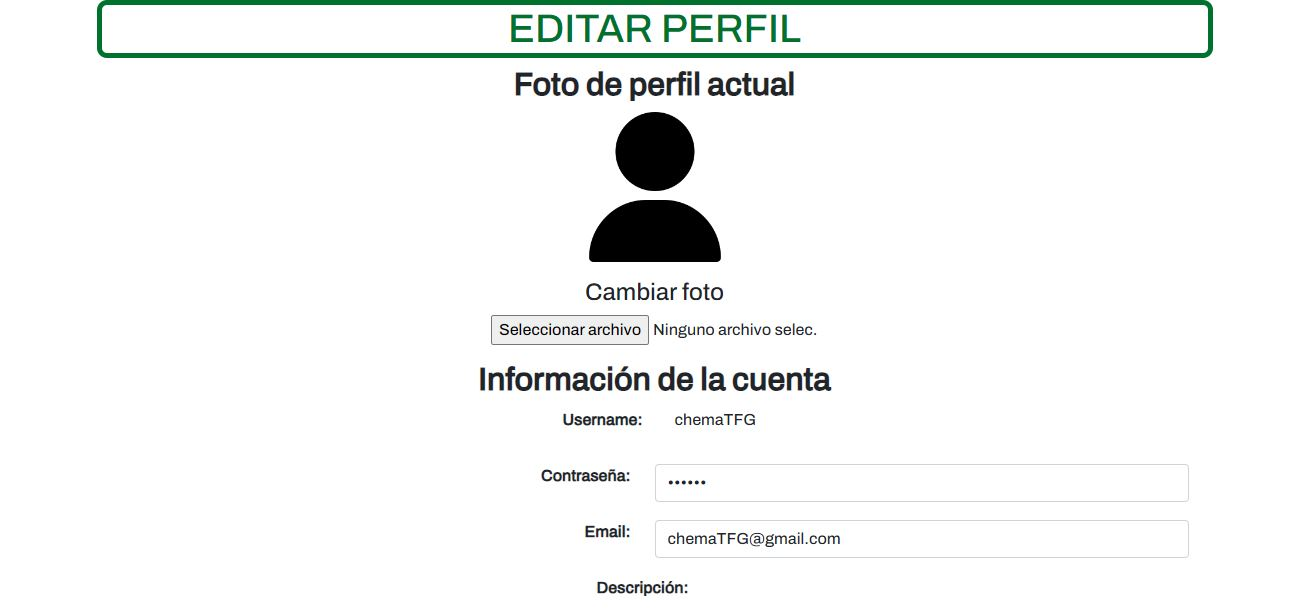
\includegraphics[scale=0.30]{img/ma-editar-perfil.JPG}
  \caption{Pantalla editar-usuario.}
  \label{fig:ma-editar-usuario}
\end{figure}

\begin{figure}
  \centering
  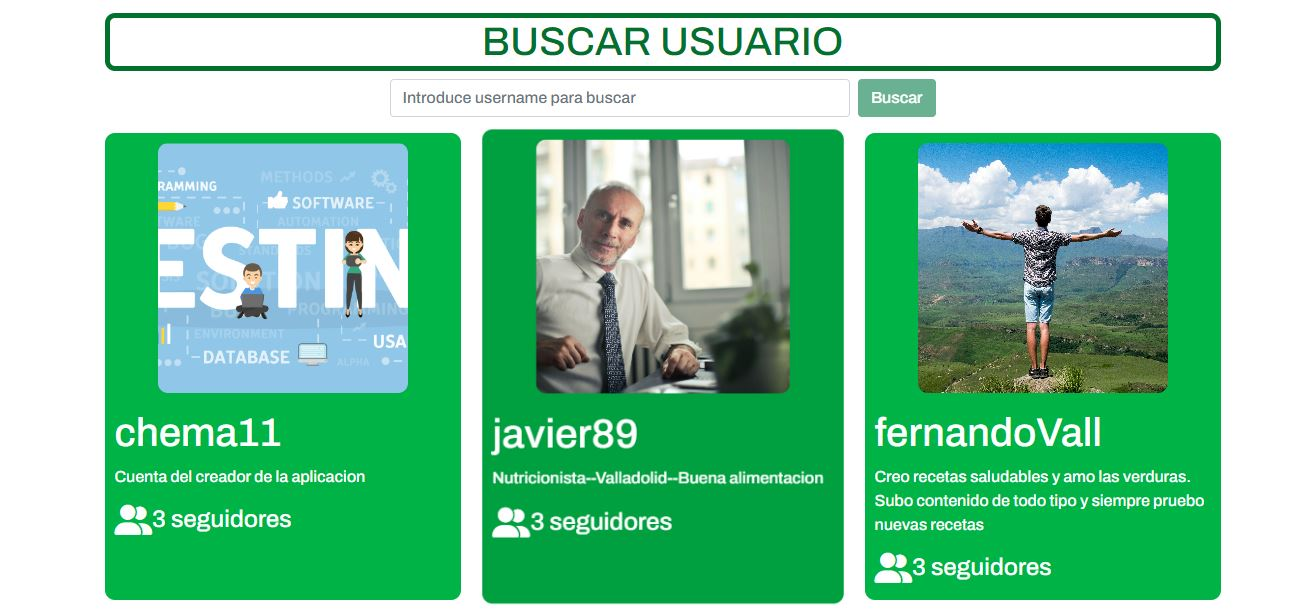
\includegraphics[scale=0.30]{img/ma-buscar-usuario.JPG}
  \caption{Pantalla buscar-usuario.}
  \label{fig:ma-buscar-usuario}
\end{figure}


\begin{figure}
  \centering
  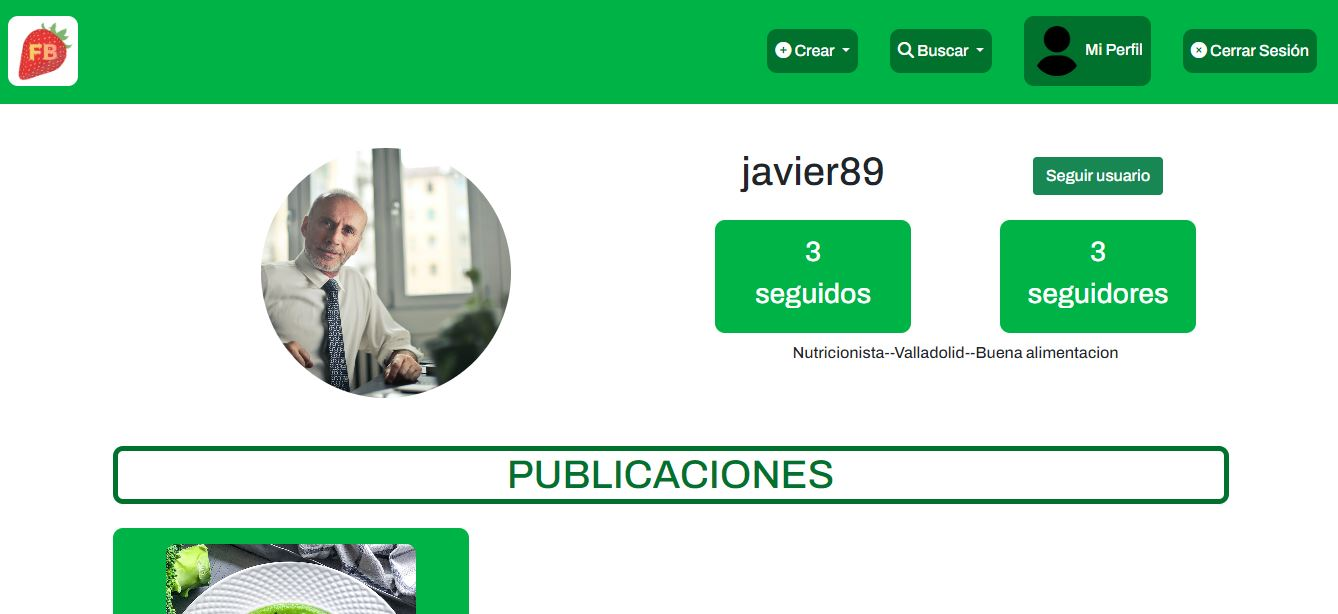
\includegraphics[scale=0.30]{img/ma-detalles-usuario.JPG}
  \caption{Pantalla detalles-usuario.}
  \label{fig:ma-detalles-usuario}
\end{figure}

\begin{figure}
  \centering
  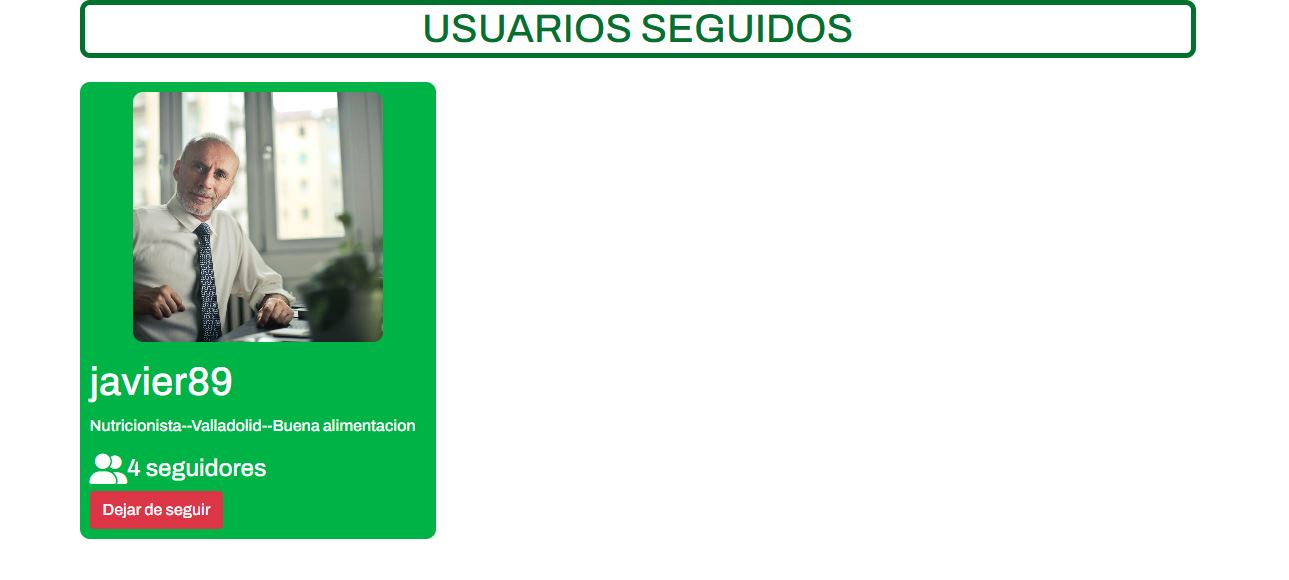
\includegraphics[scale=0.30]{img/ma-seguidos-usuario.JPG}
  \caption{Pantalla seguidos-usuario.}
  \label{fig:ma-seguidos-usuario}
\end{figure}

\begin{figure}
  \centering
  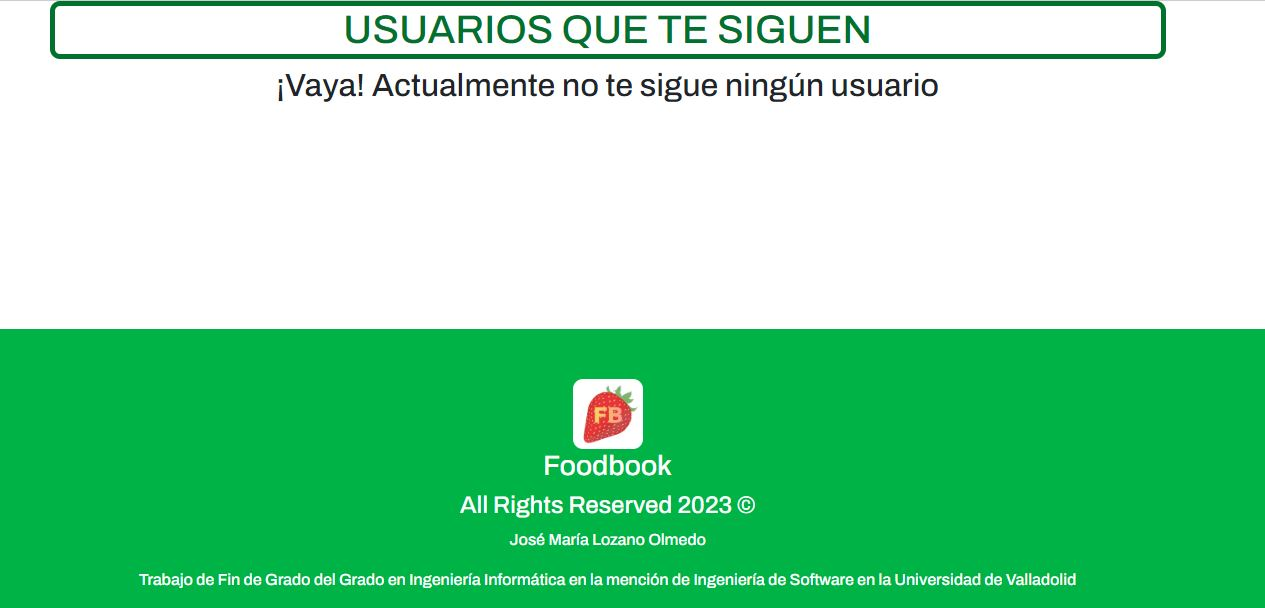
\includegraphics[scale=0.30]{img/ma-seguidores-usuario.JPG}
  \caption{Pantalla seguidores-usuario.}
  \label{fig:ma-seguidores-usuario}
\end{figure}




\begin{figure}
  \centering
  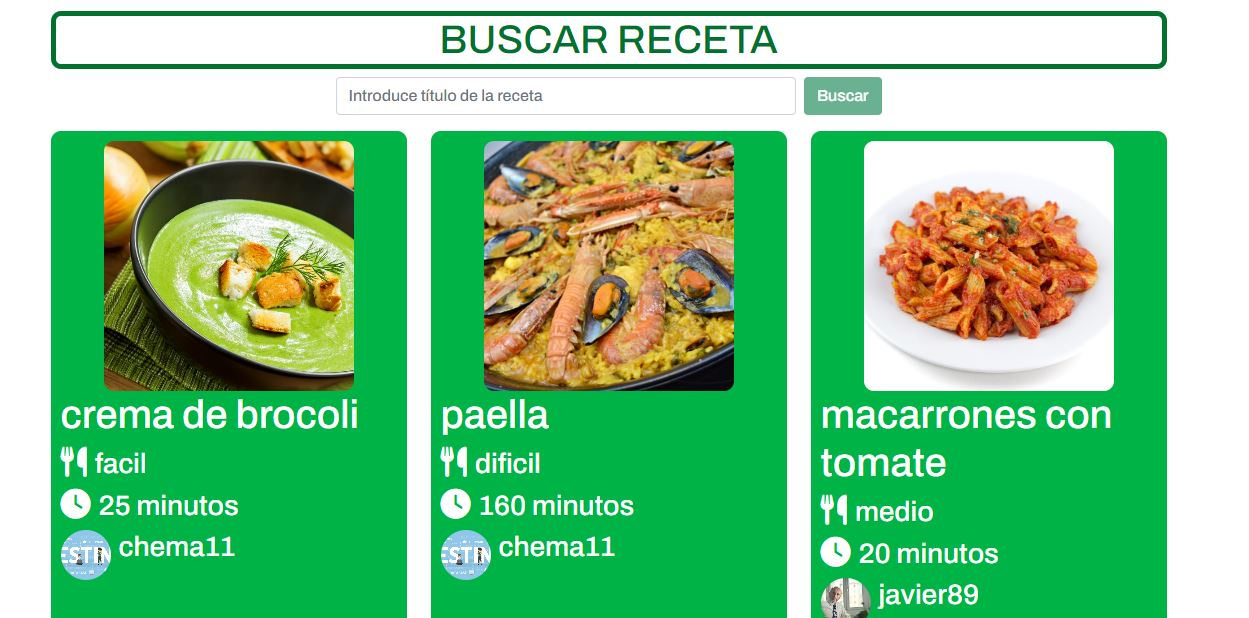
\includegraphics[scale=0.30]{img/ma-buscar-receta.JPG}
  \caption{Pantalla buscar-receta.}
  \label{fig:ma-buscar-receta}
\end{figure}

\begin{figure}
  \centering
  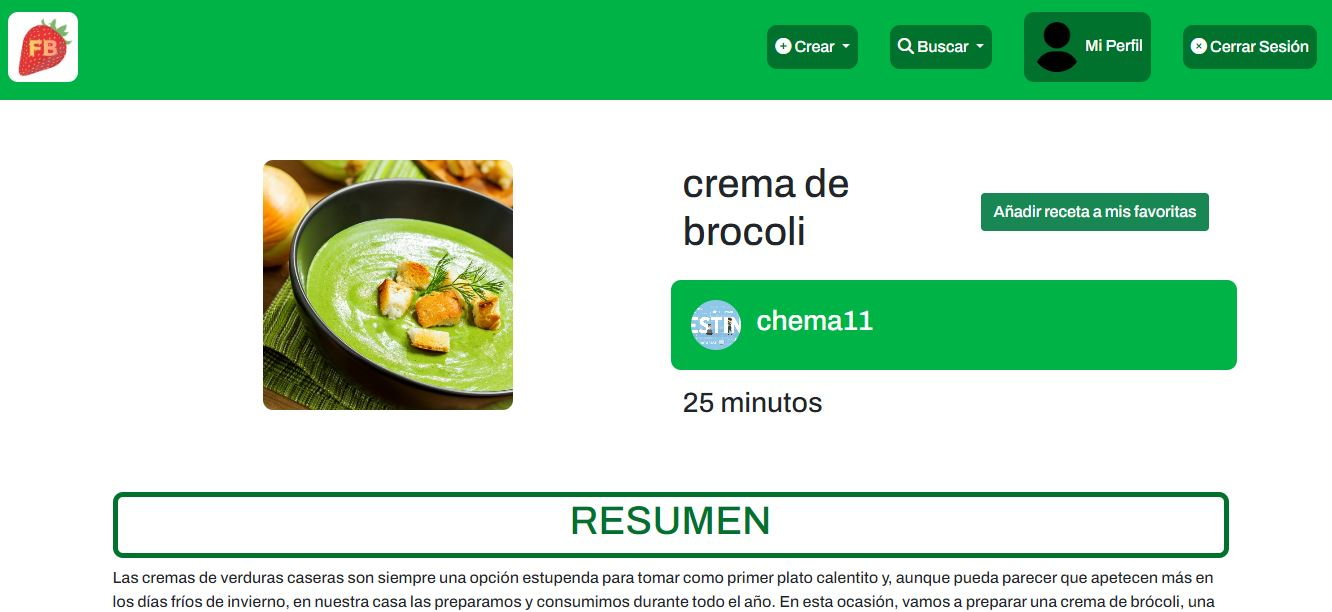
\includegraphics[scale=0.30]{img/ma-detalles-receta.JPG}
  \caption{Pantalla detalles-receta.}
  \label{fig:ma-detalles-receta}
\end{figure}

\begin{figure}
  \centering
  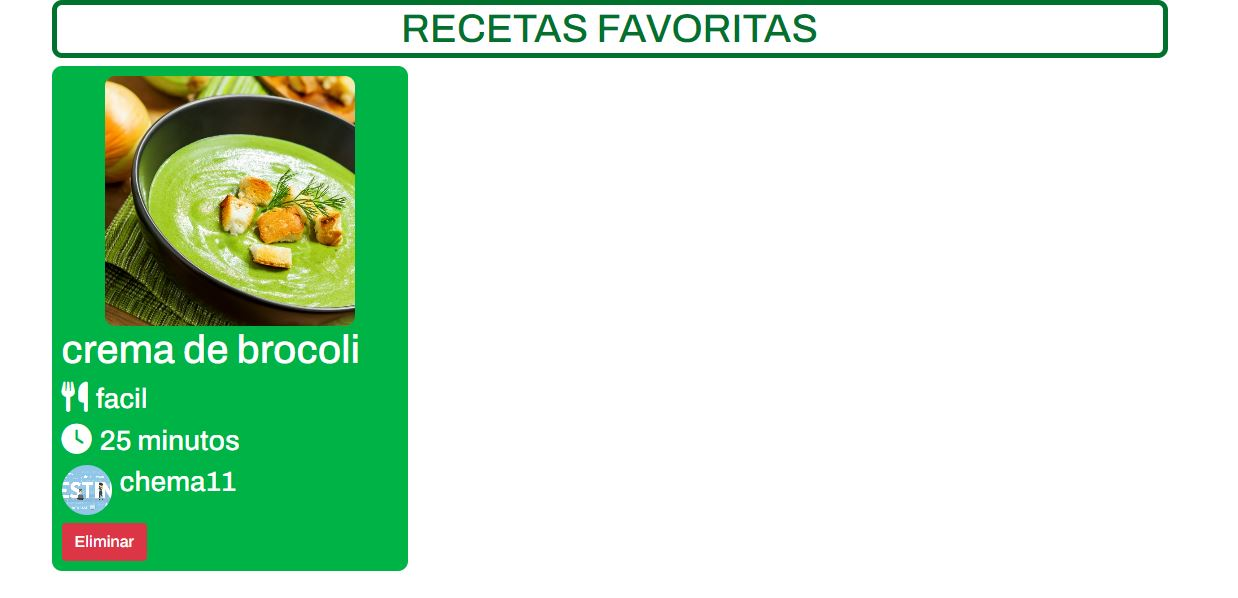
\includegraphics[scale=0.30]{img/ma-recetas-favoritas.JPG}
  \caption{Pantalla favoritas-recetas.}
  \label{fig:ma-favoritas-recetas}
\end{figure}

\begin{figure}
  \centering
  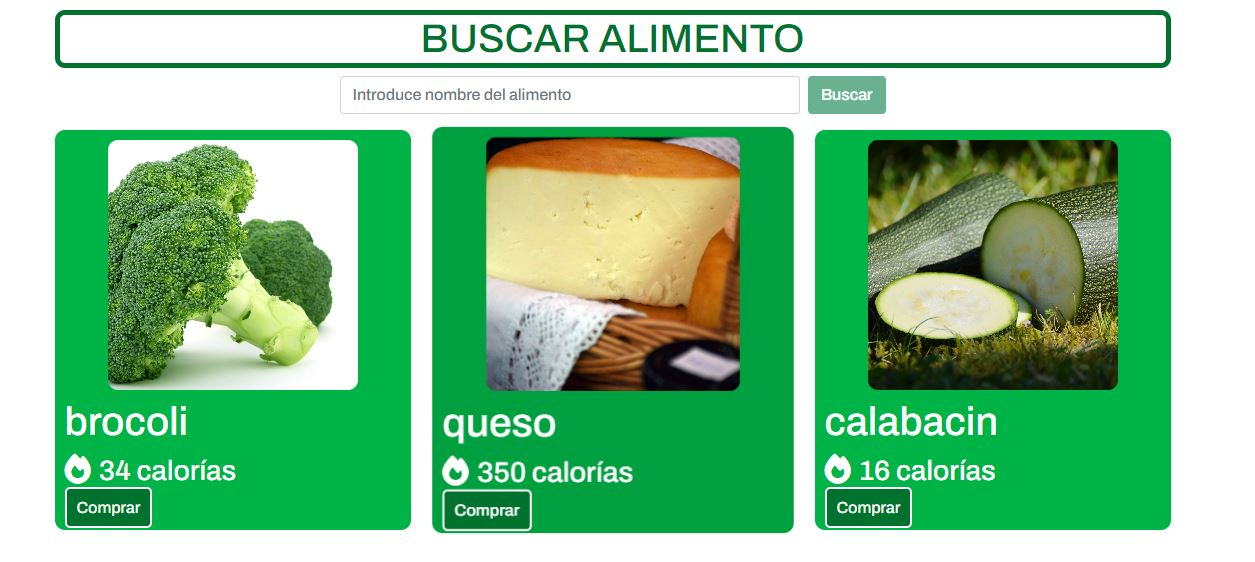
\includegraphics[scale=0.30]{img/ma-buscar-alimento.JPG}
  \caption{Pantalla buscar-alimento.}
  \label{fig:ma-buscar-alimento}
\end{figure}

\begin{figure}
  \centering
  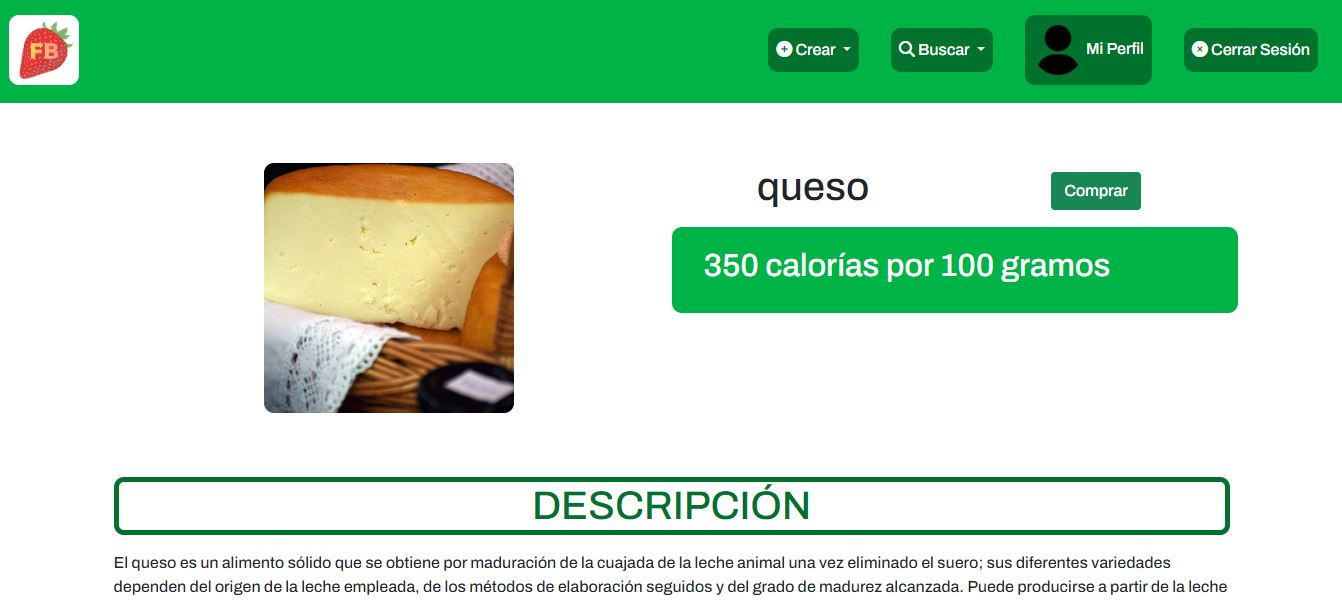
\includegraphics[scale=0.30]{img/ma-detalles-alimento.JPG}
  \caption{Pantalla detalles-alimento.}
  \label{fig:ma-detalles-alimento}
\end{figure}

\begin{figure}
  \centering
  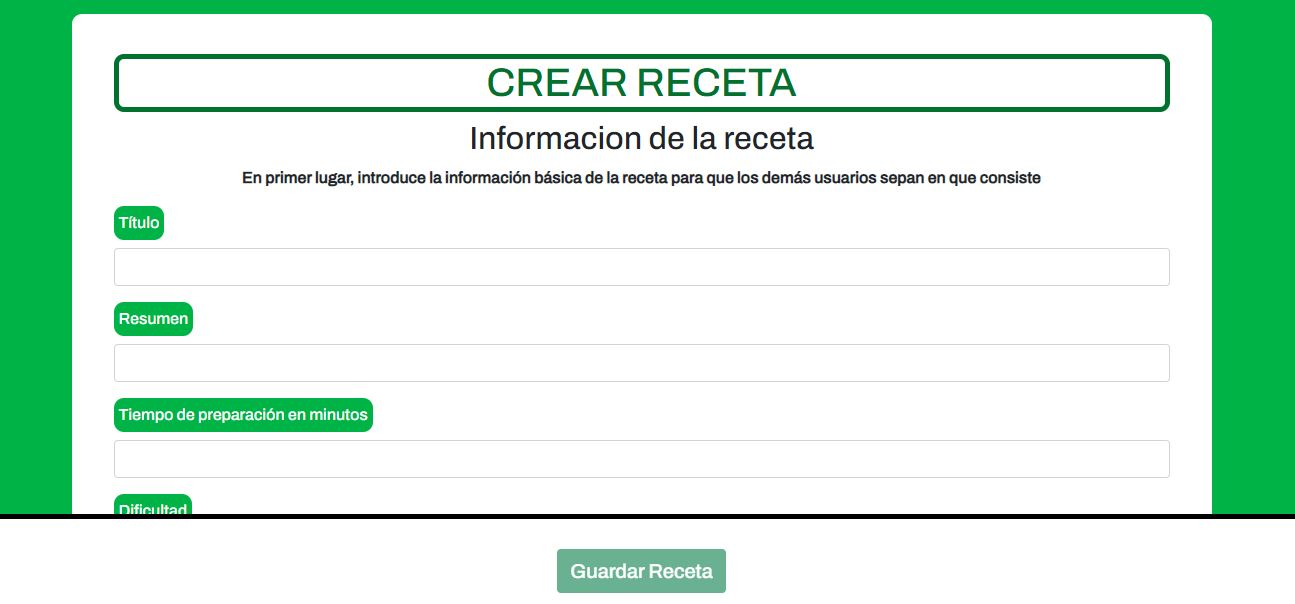
\includegraphics[scale=0.30]{img/ma-crear-receta.JPG}
  \caption{Pantalla crear-receta.}
  \label{fig:ma-crear-receta}
\end{figure}

\begin{figure}
  \centering
  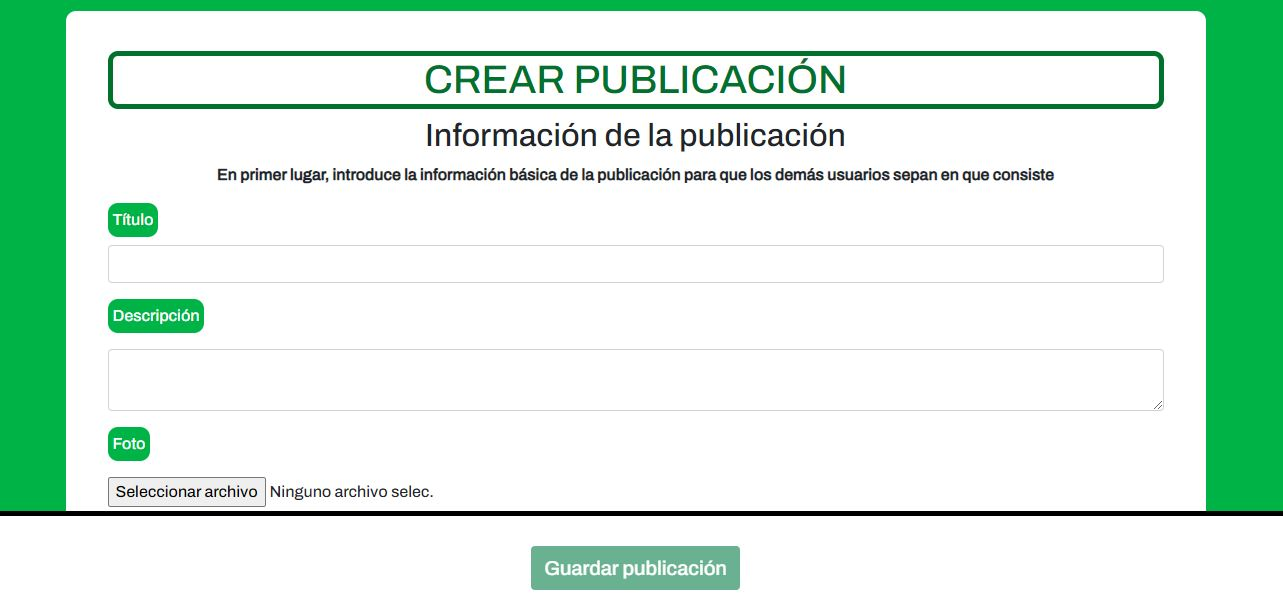
\includegraphics[scale=0.30]{img/ma-crear-publicacion.JPG}
  \caption{Pantalla crear-publicacion.}
  \label{fig:ma-crear-publicacion}
\end{figure}

\begin{figure}
  \centering
  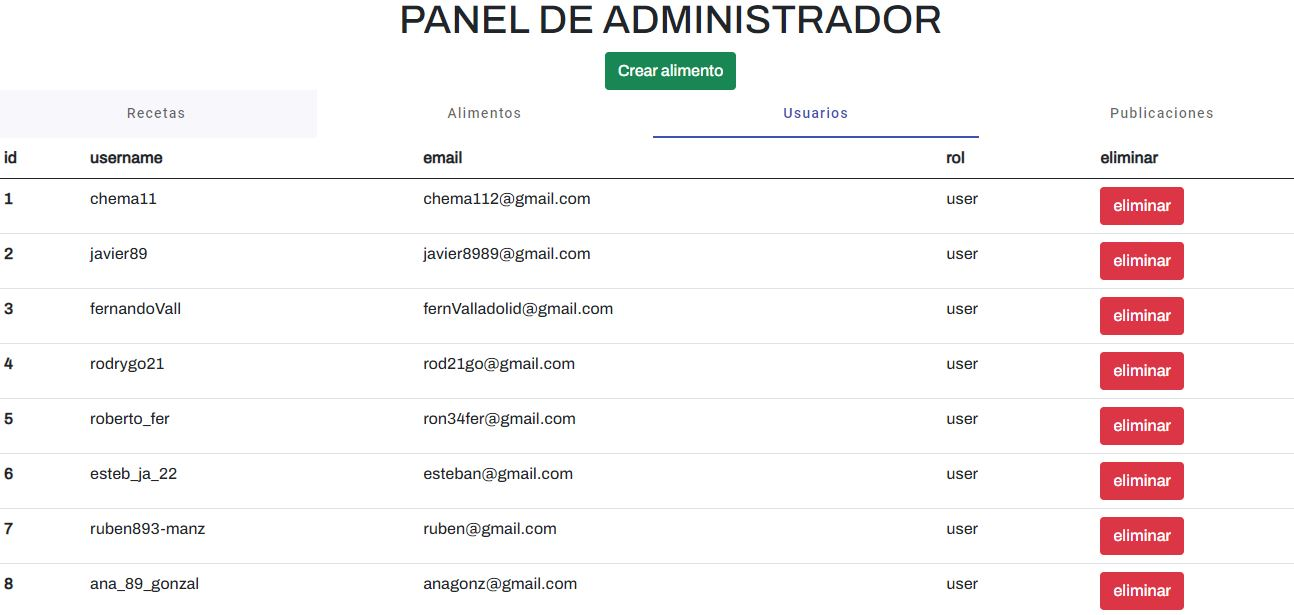
\includegraphics[scale=0.30]{img/ma-usuarios-admin.JPG}
  \caption{Pantalla vista-admin en la pestaña usuarios.}
  \label{fig:ma-usuarios-admin}
\end{figure}

\begin{figure}
  \centering
  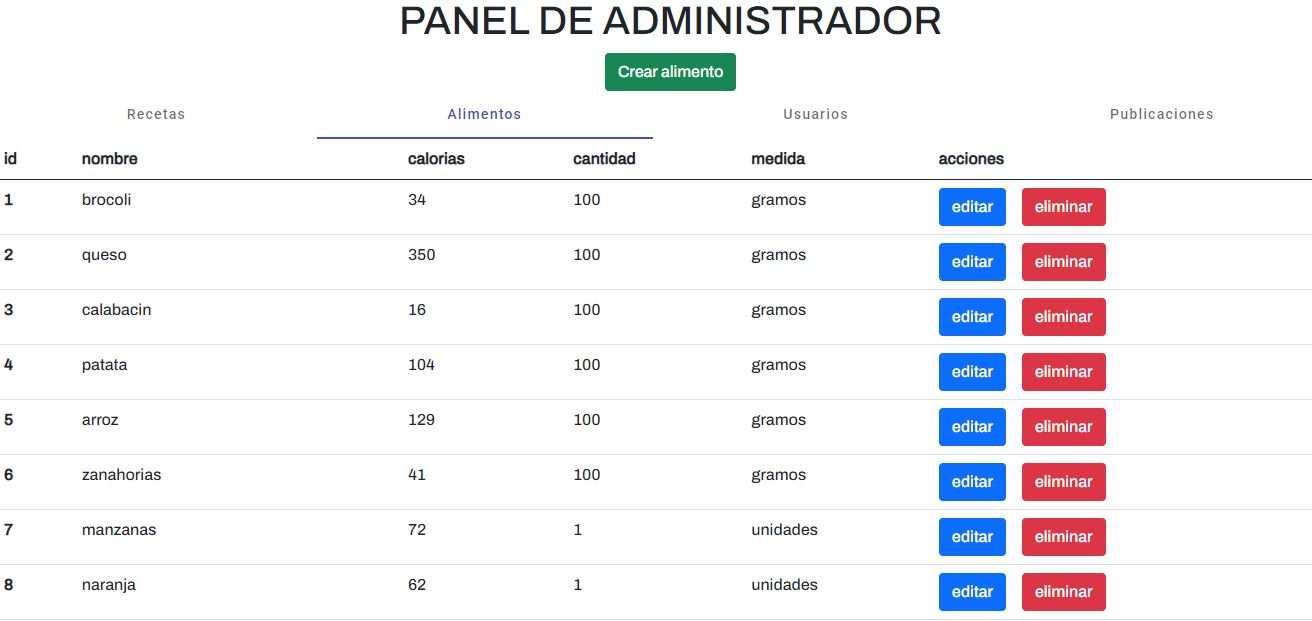
\includegraphics[scale=0.30]{img/ma-alimentos-admin.JPG}
  \caption{Pantalla vista-admin en la pestaña alimentos.}
  \label{fig:ma-alimentos-admin}
\end{figure}

\begin{figure}
  \centering
  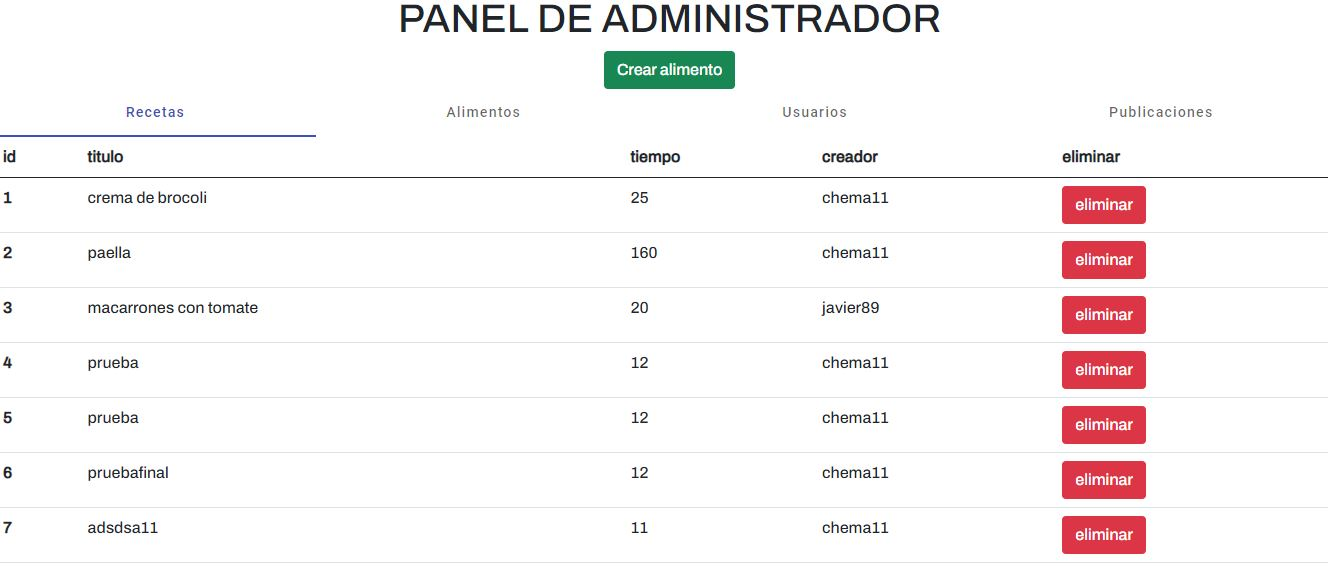
\includegraphics[scale=0.30]{img/ma-recetas-admin.JPG}
  \caption{Pantalla vista-admin en la pestaña recetas.}
  \label{fig:ma-recetas-admin}
\end{figure}

\begin{figure}
  \centering
  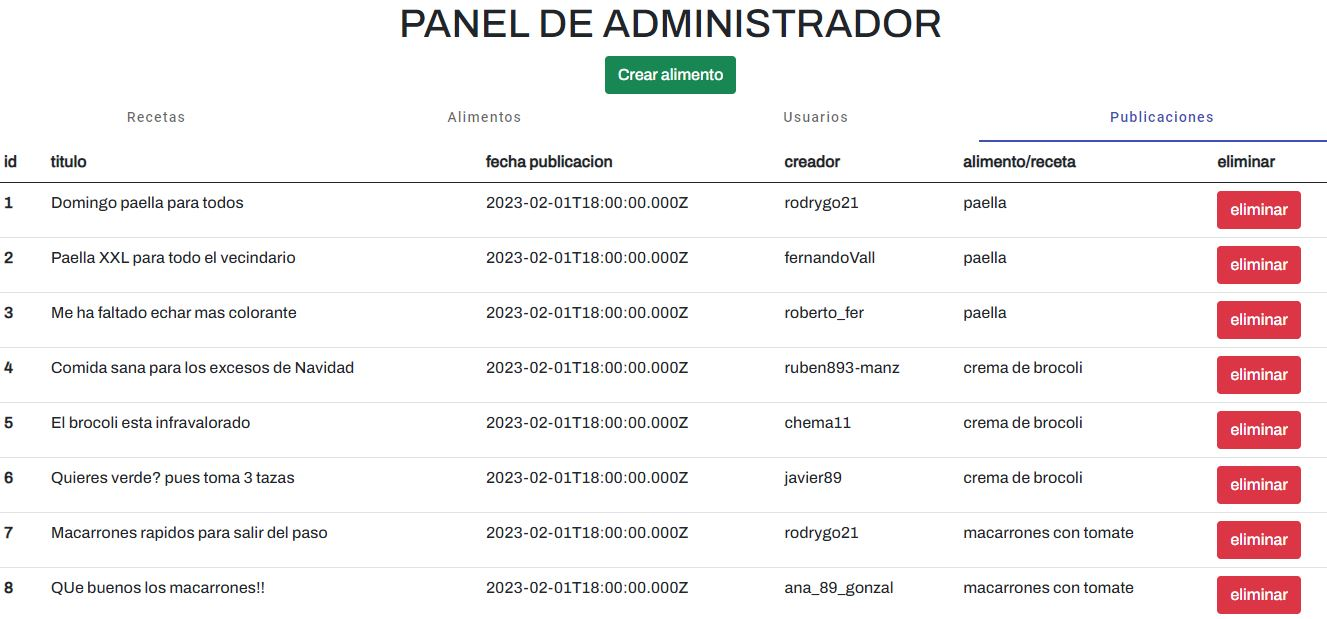
\includegraphics[scale=0.30]{img/ma-publicaciones-admin.JPG}
  \caption{Pantalla vista-admin en la pestaña publicaciones.}
  \label{fig:ma-publicaciones-admin}
\end{figure}




\begin{figure}
  \centering
  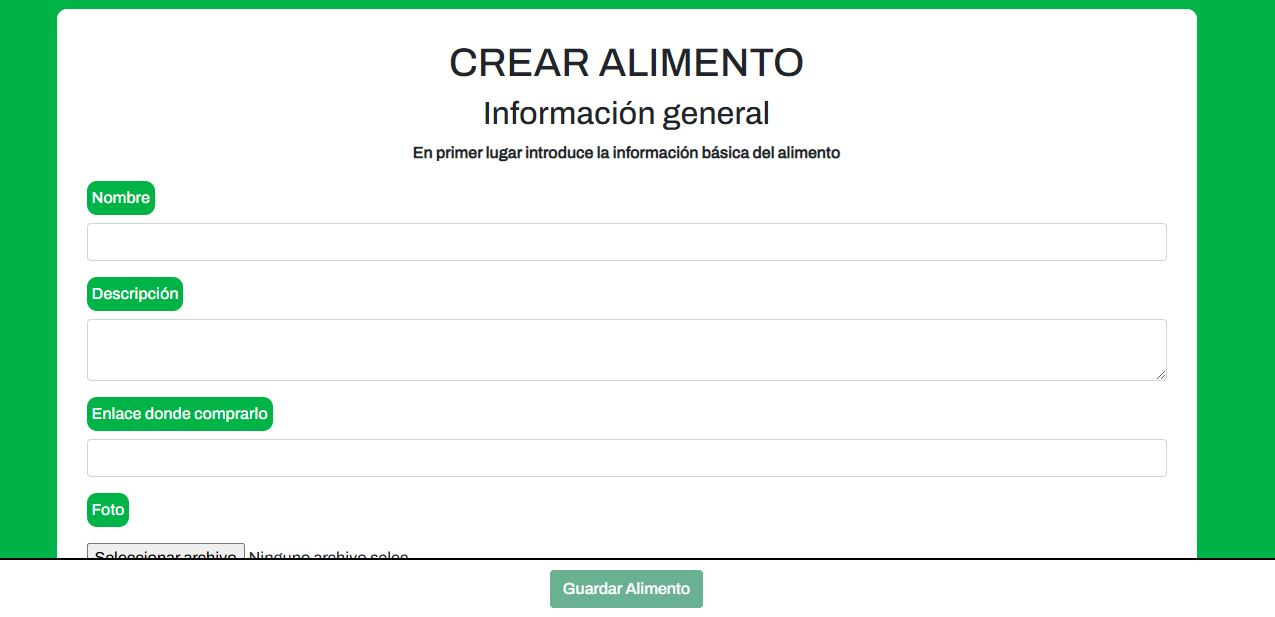
\includegraphics[scale=0.30]{img/ma-crear-alimento.JPG}
  \caption{Pantalla crear-alimento.}
  \label{fig:ma-crear-alimento}
\end{figure}

\begin{figure}
  \centering
  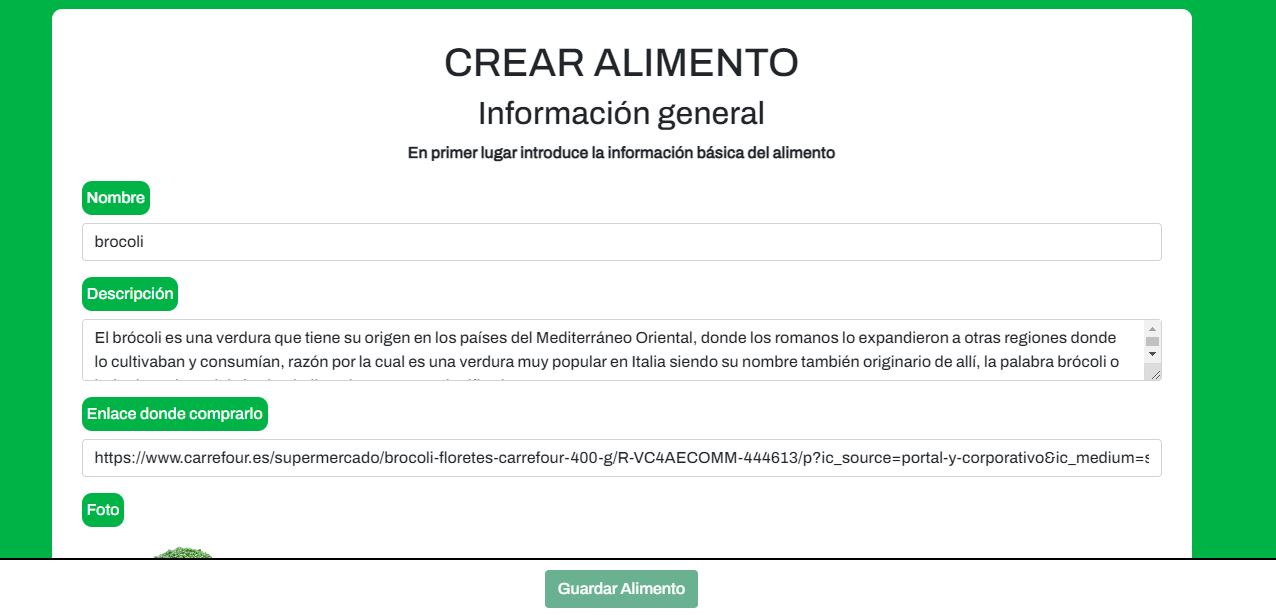
\includegraphics[scale=0.30]{img/ma-editar-alimento.JPG}
  \caption{Pantalla editar-alimento.}
  \label{fig:ma-editar-alimento}
\end{figure}